\section{Architecture}
\label{section:architecture}

The overall architecture which we have implemented in Mininet framework is 
shown in Figure~\ref{fig:arch}. The architecture of the distributed L3-VPN 
network is of hub-and-spoke type. Hub nodes comprise the backbone of the network,
whereas, multiple spoke PE elements are attached to the hubs. This allows to
achieve scalability property. The security of the network is achieved by using 
Host Identity Protocol to negotiated the authentication keys, whereas, actual
packet authentication is performed on hop-by-hop bases using HMAC-SHA256 algorithm~\cite{Stinson:Cryptography}. 

The Mininet prototype is available online and can be found in GitHub~\cite{l3vpn}.

\begin{figure}[!h]
	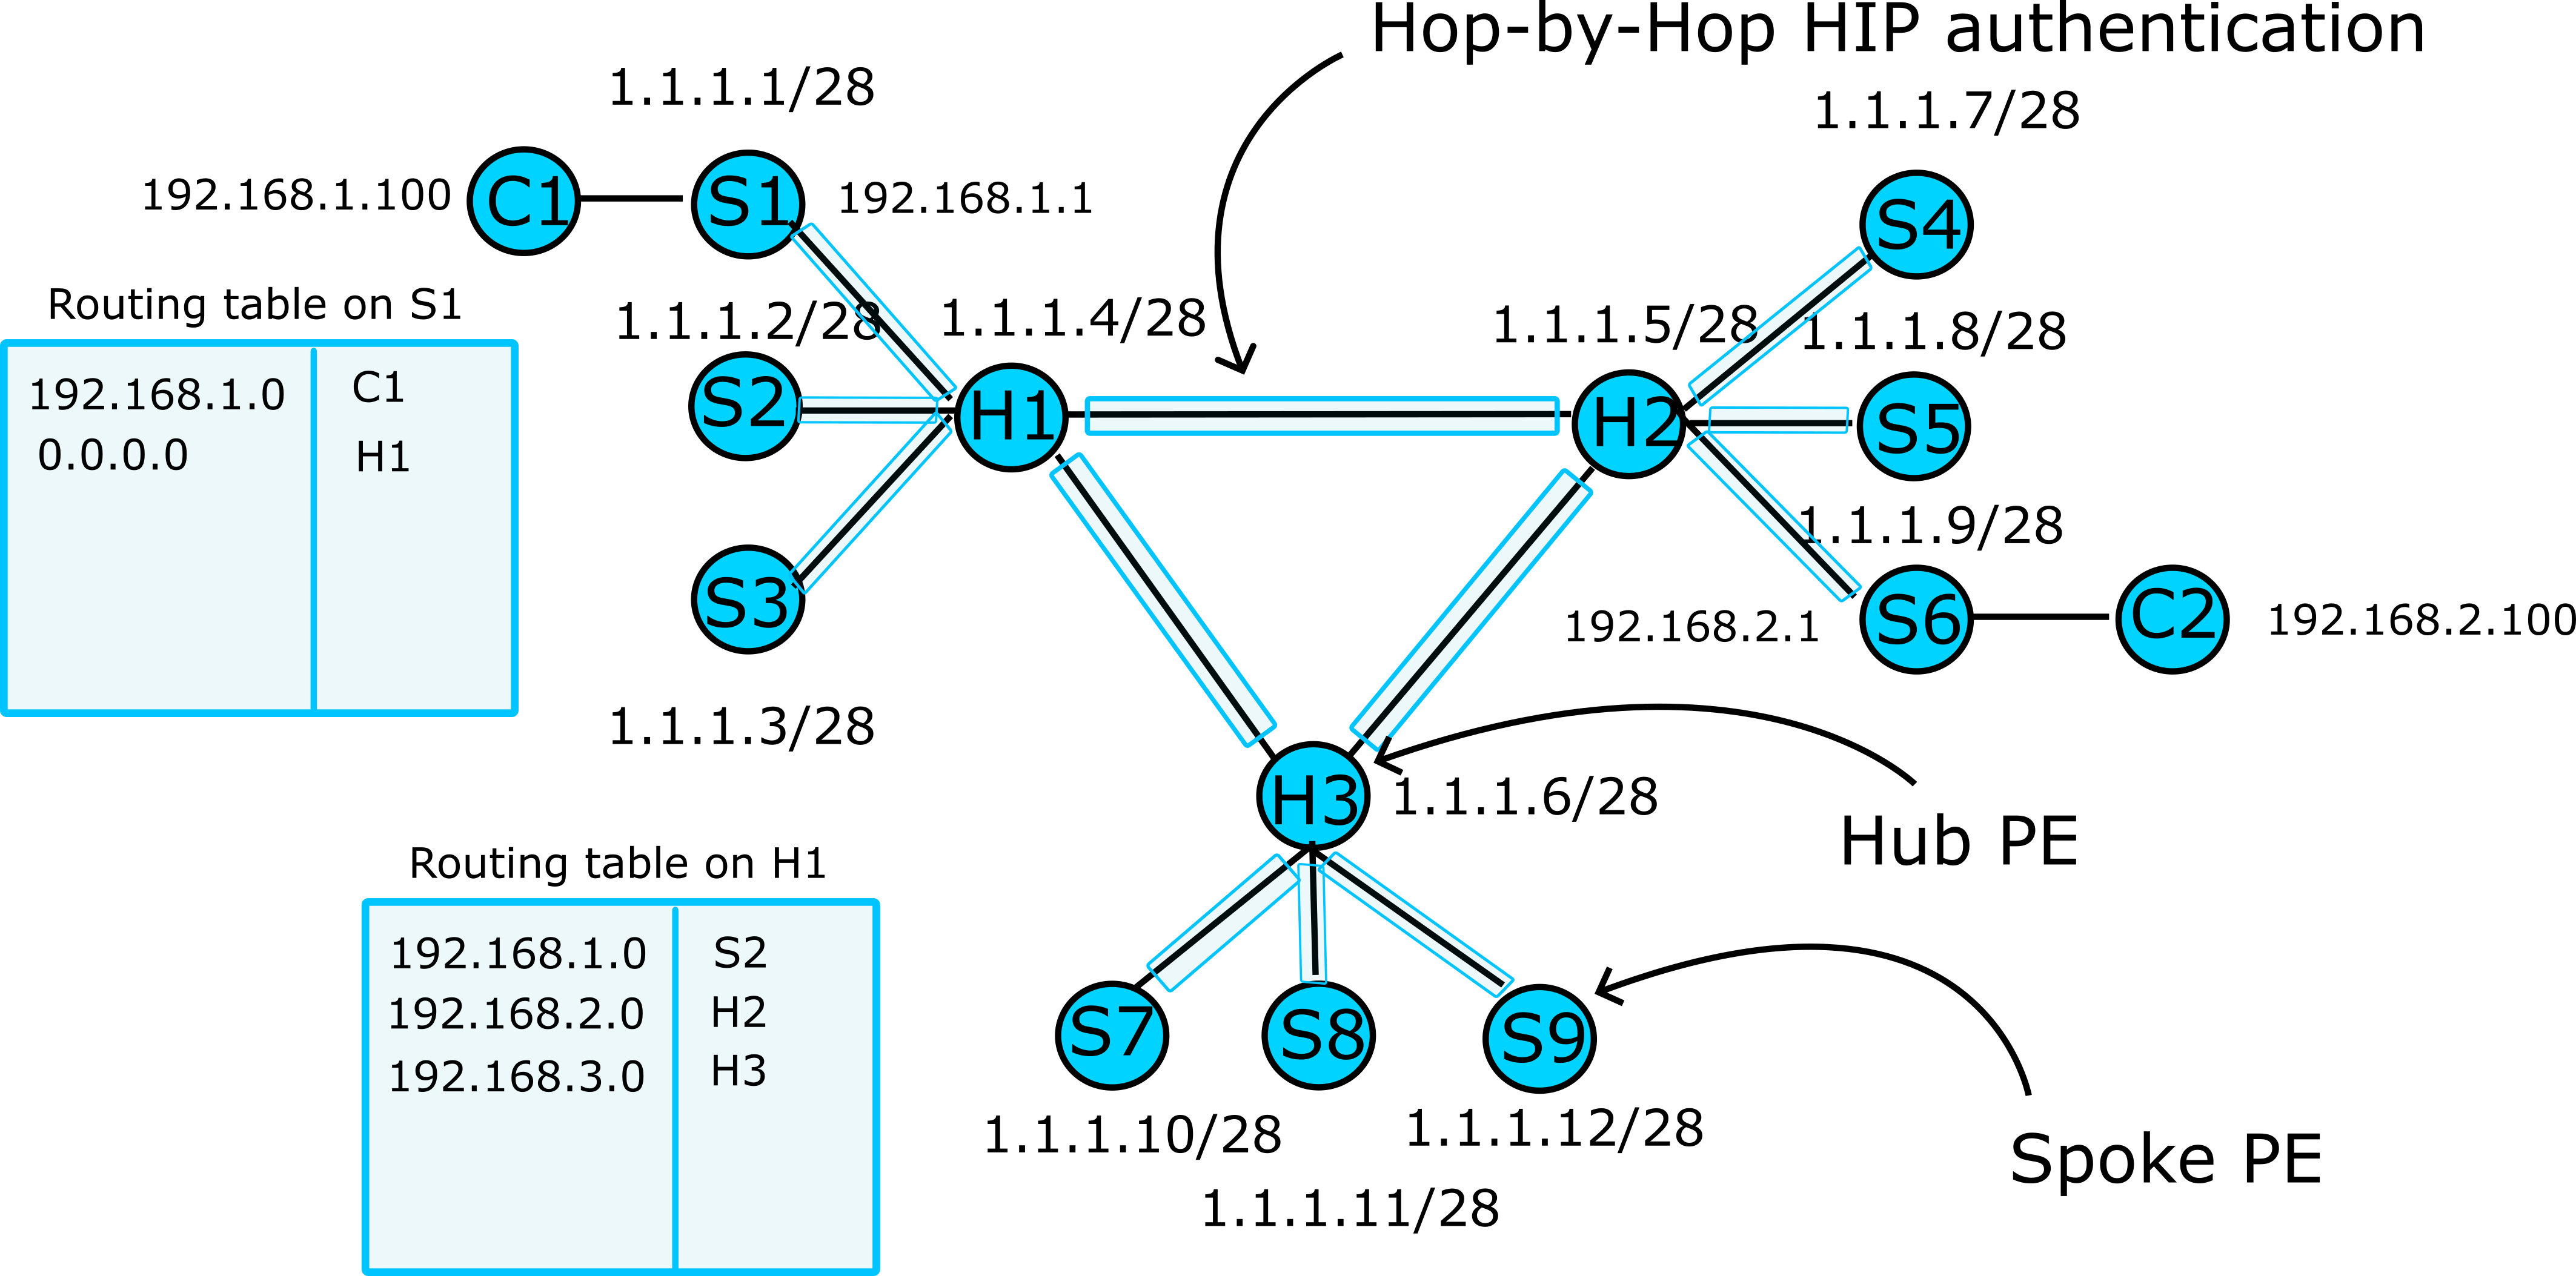
\includegraphics[width=0.5\textwidth]{graphics/arch.png}
	\caption{High-level architecture of L3-VPN deployed in Mininet}
	\label{fig:arch}
\end{figure}

\begin{table*}
        \begin{tabular}{|l|c|c|c|}
        \hline
        Characteristic $\downarrow$ \ Overlay type $\rightarrow$ & L2-VPLS & L3-VPN & HIP-VPLS~\cite{hipvpls} \\\hline
        Size of forwarding/routing table & $O(n)$, $n$-number of hosts & $O(m)$, $m$ - number of subnetworks & $O(n)$\\\hline
        Number of links in mesh & $O(k^2)$, $k$ - number of Hub-PEs & $O(k^2)$ & $O(l^2)$, $l$ - number of PEs \\\hline
        Privacy & MACs are exposed to PEs & IPs are exposed to PEs & No exposure of MACs and IPs (PEs are part of customers infrastructure) \\\hline
        Encryption and authentication & Hop-by-hop & Hop-by-hop & End-to-end \\\hline
        Tunneling mode & Ethernet-in-IP & IP-in-IP & Ethernet-in-IP \\\hline
        Loop free-topology & 802.1d protocol/central controller & Central controller & Not required \\\hline
        \end{tabular}
        \label{tab:analysis}
        \caption {Comparison study of different multipoint VPLS/VPN designs}
\end{table*}


